\section{Energetic particles in the heliosphere}
\label{sec:particles_heliosphere}


The heliosphere is a vast, bubble-like region in space that envelops the Sun. This region is moving with respect to the \ac{ISM} with a speed of about 25 km/s \citep{McComas2015ApJS}. It is also a plasma cavity that is created by the Sun and is governd by the solar wind and its magnetic field; a substantial amount of plasmas of various particle populations fill this space. The particle populations are identified from Fig.\ref{Fig:Oxygen_spectra_heliosphere} which is adapted from \citet{Mewaldt-2001}. Based on the accumulated measurements of oxygen by the \ac{ACE} between 1997 and 2000 at 1 au, the oxygen fluence spectrum which spans over more than seven orders of magnitude from keV/nuc to GeV/nuc provides clear insight into the lower energy particles including the slow solar wind, the fast solar wind, the suprathermal tails, and high energetic particles composed of \acp{SEP}, \acp{ACR}, and the extremely high energetic \acp{GCR}. 

%Among them \acp{GCR} originate from distant sources outside the solar system, while \acs{ACR} sources are located near the boundary of the heliosphere. The remaining energetic particles are accelerated and generated inside of the heliosphere at the multiple locations, including the solar surface, interplanetary space and even the planets, for instance Jupiter.

\begin{figure}[!htb]
	% moving the figure to the second page
	\centering
	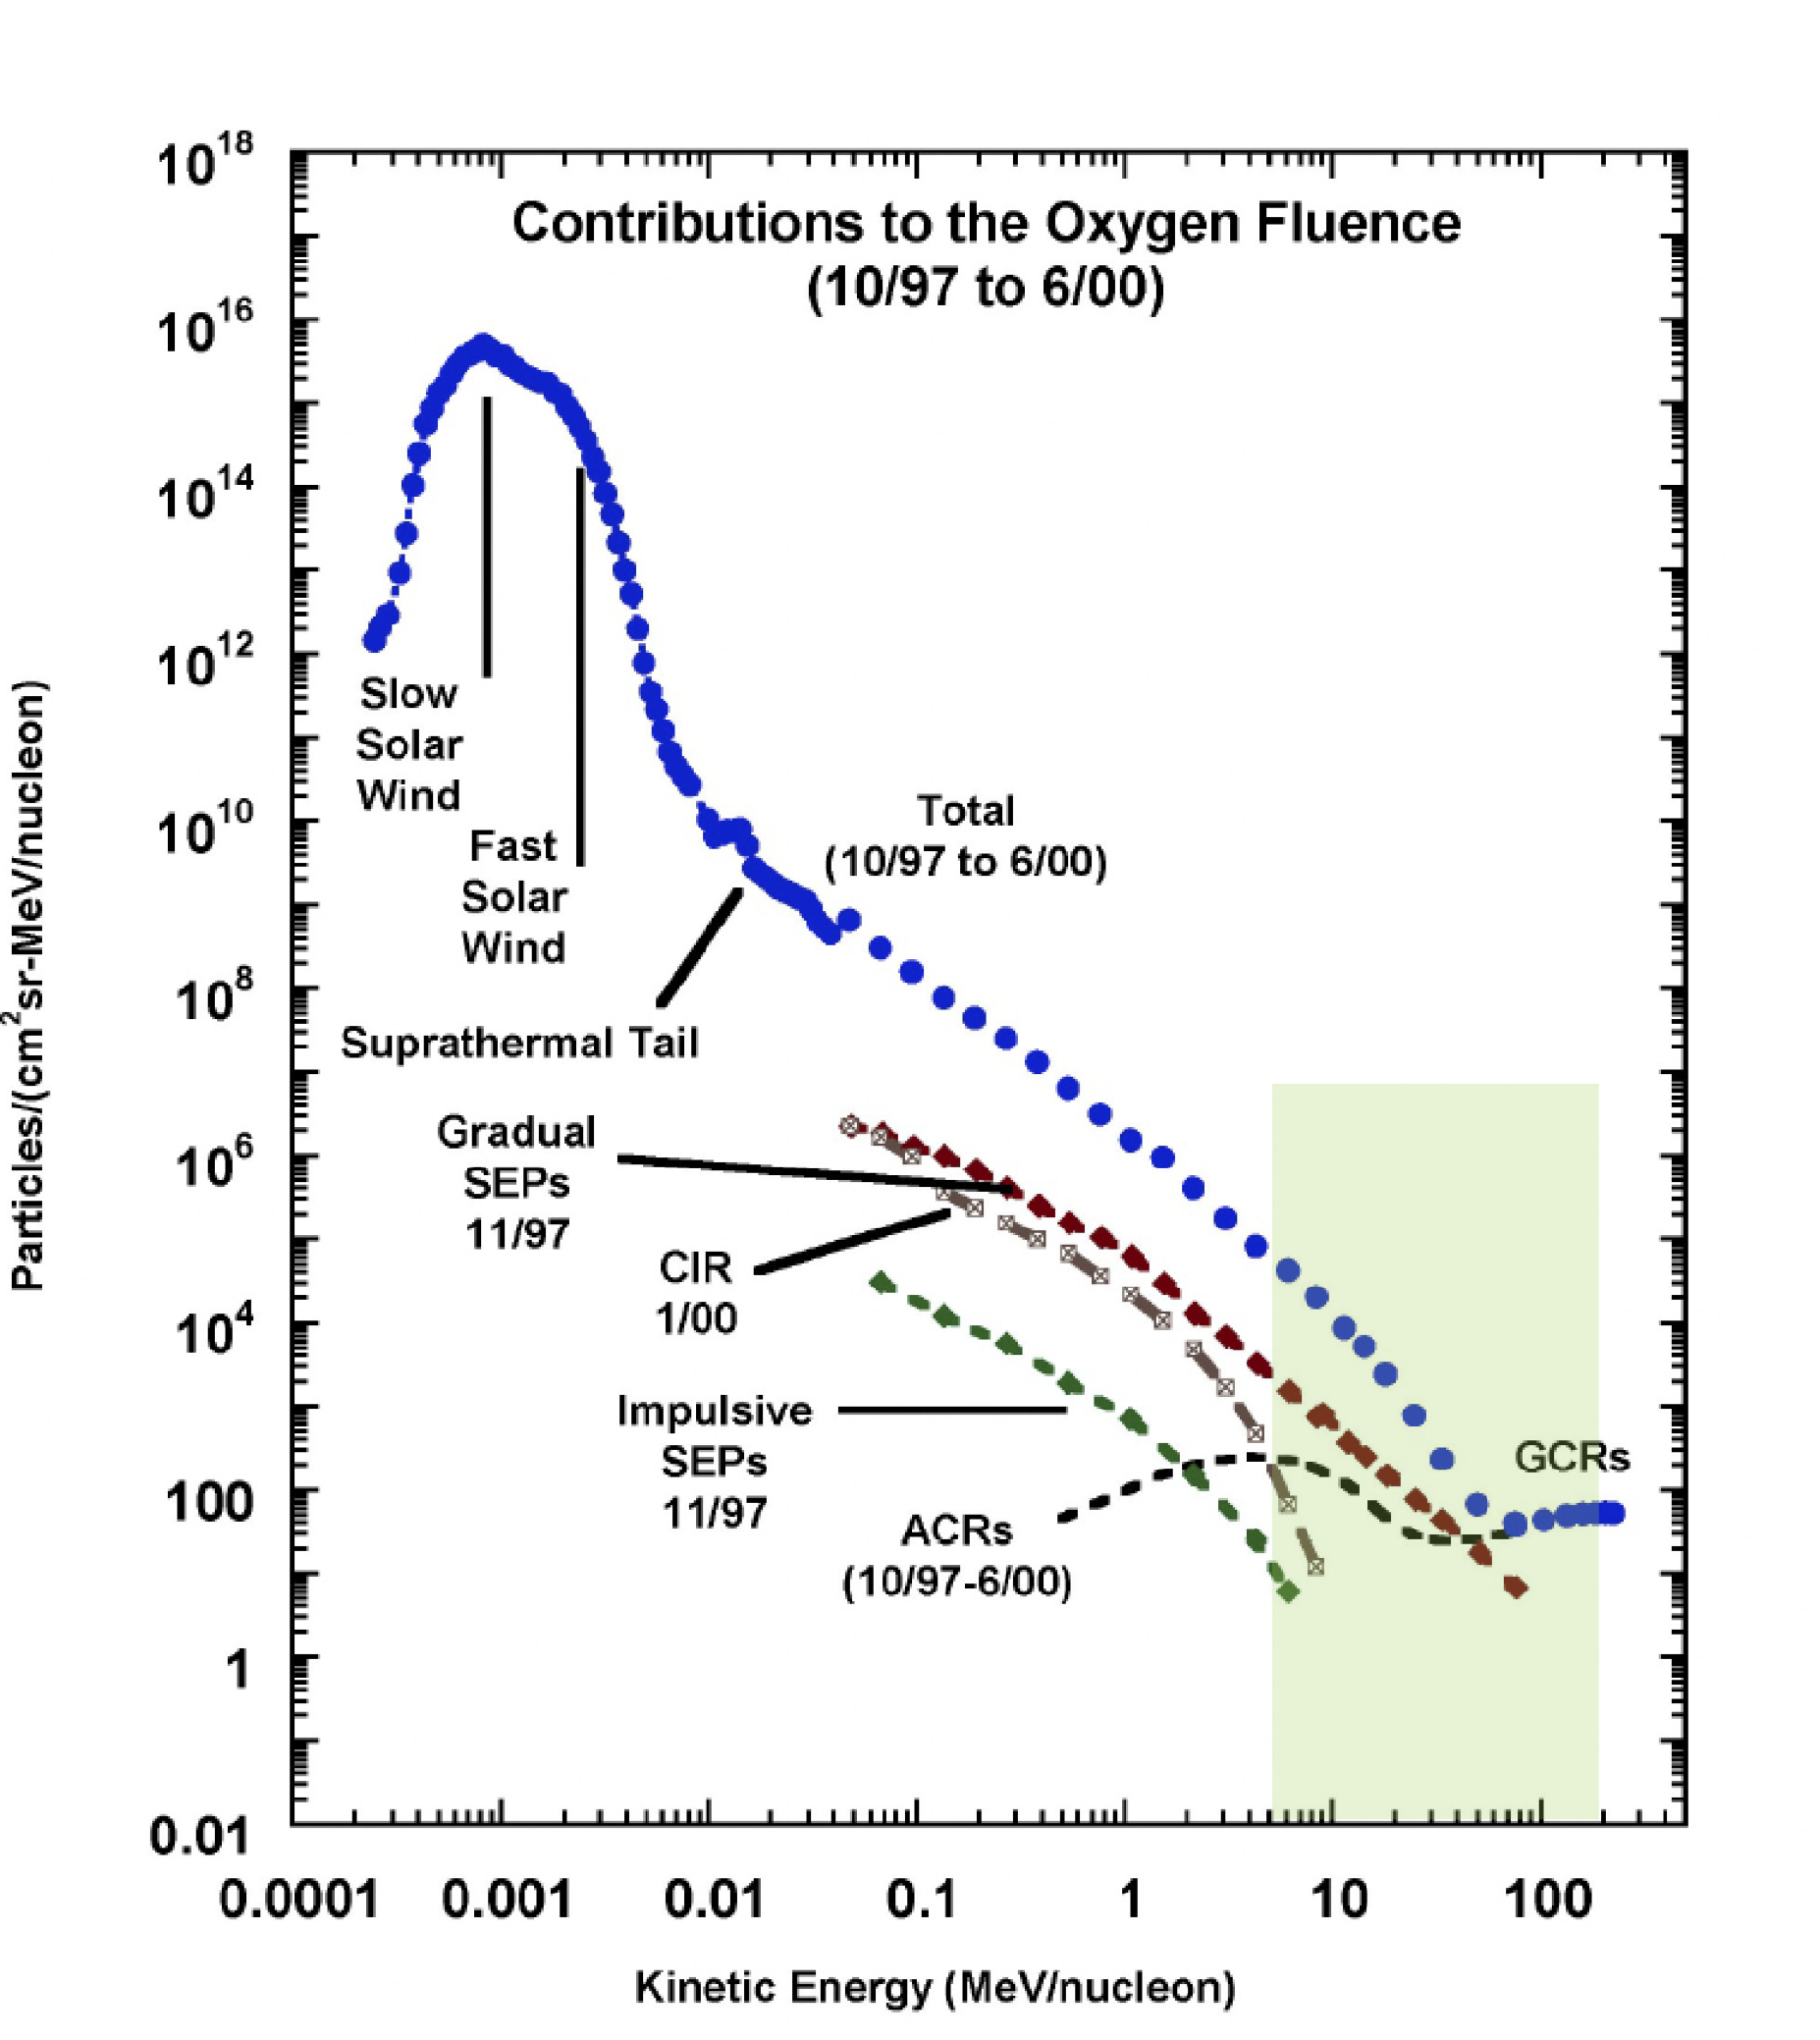
\includegraphics[width = 0.8\textwidth]{images/heliospheric_particle_spectra_color.png}
	\caption[Energy spectra of oxygen ions in near-Earth space]{The typical oxygen spectra in the interplanetary space near Earth, indicating the contributions of different particle populations, particularly in the energy range between few MeV/nuc and few hundreds MeV/nuc (green shaded region), where \acs{SEP}, \acs{ACR} and \acs{GCR} coexist. The spectra of other particle species such as, helium and protons have a similar shape but a different flux level in the corresponding energy regime. The figure is adapted from \citep{Mewaldt-2001}}
	\label{Fig:Oxygen_spectra_heliosphere}
\end{figure}


The solar wind is a stream of charged particles released from the solar corona, the upper atmosphere of the Sun. This plasma consists of mainly protons and electrons that continously flow outward and expand to about $\sim$ 100 au (depending on the direction and the phase of solar activity cycle). The typical energy range of the solar wind is between 0.5 keV and 4.5 keV. Depending on the locations that produce the solar wind, the speed and density of the solar wind might be different. For instance the fast solar wind with a typical speed between 500 and 800 kilometers per second is emitted from the coronal holes which are funnel-like regions of open field lines in the magnetic field and usually appear at the north and south pole of the Sun \citep{Sakao2007, Tu2005, hundhausen1968state}. Therefore, the fast solar wind dominates the high latitude regions. On the other hand, the slow solar wind is observed to have a velocity of about 300 - 500 kilometers per second and is believed to originate from the streamer belt along the equatorial belt. The slow solar wind is more likely to be observed in the low latitude regions.


%plasma embedding with magnetic field

Suprathermal particles are charged ions and electrons that move about two to hundreds times faster than the solar wind particles. In the spectrum shown in Fig.\ref{Fig:Oxygen_spectra_heliosphere}, the suprathermal particles are beyond the tails of the fast solar wind and are the dominant particle population between few keV to hundreds of keV. The source of the suprathermal particle might be accelerated solar wind and the remanent of the previous solar eruptions and \ac{SEP} events \citep{Gloeckler1995SSRv}. Suprathermal particles are suspected to play an important role as seed particles for \ac{SEP} events \citep{Kahler2019ApJ}.
%Those particles play an important role in contributing seed particles for \ac{SEP} events.

Above the energy of suprathermal particle is the energy range that we are interested in this thesis, especially the energy range between 10 MeV/nuc and few hundred MeV/nuc where the dominant particles are \acp{SEP} (not limited to this energy range), \acp{ACR} (up to $\sim$ 100 MeV/nuc) and lower energy \acp{GCR}. The measurements we used in this study are from this energy range.

\acp{SEP} are high energetic particles with energies ranging from few keV up to $\sim$ GeV. They are emitted from the Sun and accelerated by solar flares and \ac{CME}-driven shocks. \acs{SEP} events are intermittent, short term, and normally intensive, compared with cosmic rays \citep{Reames1999}. Different type of \acs{SEP} events persist for different time scales from few hours to few days. Such high energy particles are one of the major threats in the space.
%also particle from solar, accelerated by different mechanism. The enery range of \ac{SEP} are quite broad, especially depending the on where the measurement carried on. Recently \ac{SOLO} and \ac{PSP} frequently measure the hundreds keV \ac{SEP}.

\acs{ACR} are believe to be the high energy interstellar pick-up ions \citep{Giacalone2022SSRv} which are neutral interstellar atoms ionized by solar UV radiation after neutral atoms move cross the boundary and enter the heliosphere. Those ionized particle are then carried by the expanding solar wind to the outer boundary of the helioesphere, where they are accelerated by the termination shock and then propagate inwards. The typcial \ac{ACR} species that have been observed are proton, helium, oxygen, nitrogen, iron and neon. 

\acp{GCR} are the fully ionized particles that are accelerated at the so-called supernova remnants \citep{Blasi2013AARv2013} outside of the solar system. Those high energy particles bombard Earth in a constant and slowly varying way. The complete GCR spectrum cover the energy from typical 1MeV \citep{Potgieter2013LRSP} to ZeV which is larger than the energy range in Fig.~\ref{Fig:Oxygen_spectra_heliosphere}. \acp{GCR} are comprised of about 89\% of hydrogen, 10\% of helium, 1\% of heavier ions as well as electrons, positrons and antiprotons. 

After entering the heliosphere, the transport of both \acp{ACR} and \acp{GCR} are controled by the \ac{HMF}, hence \ac{ACR}'s and \ac{GCR}'s temporal variaton is highly related to the solar activity and the so-called solar modulation. More details of the solar modulation will be discussed in Section \ref{Sec:GCR}.


% LND and SOLO/EPD are new instruments;

% In the helioshphere, 

% Questions:


% 0. Cross calibrate the new data from new instrument; how is the performance of the new instrument? Are they good enough? - To answer this question
% 1. How the widespread SEP generated



\section{Motivation}
But, why we choose energetic particles in the tens of MeV/nuc range as the central topic of this thesis? First of all, it is worth noting that charged particles within this energy range exhibit complicated properties and consist of three distinct particle populations, which vary depending on time, energy range and particle species. The task of disentangling the specific particle types within this energy range is extremely challenging, especially during the solar active period.
By investigating these charged particles, we have the oppurtunity to gain insights into the origin, acceleration and transport mechanisms of \acp{SEP}, \acp{ACR} and \acp{GCR}.

Furthmore, as the space exploration continues to advance, particles in the tens of MeV/nuc are recognized as one of the most dangerous radiation in the space and pose potential threats to both astronaut health and the functioning of electronic devices. Therefore, understanding the variations and distribution of those energetic particles in the space is of particular importance for the future human space exploration.

Lastly, another compelling reason for selecting is the new data from two instruments, \ac{LND} on board Chang/E-4 and \ac{HET} on board \ac{SolO}, which were developed by the Kiel university and measure charged particles within this energy range. \ac{LND} is the first human mission on the far-side surface of Moon and serves as a monitor of the radiation environment and a charged particle telescope. Meanwhile, \ac{HET} provides the excellent oppurtunity to measure energetic particles within 1 au. Analyzing these new measurements allows for a reassessment of the various aspects related to tens of MeV/nuc energetic particle in the new solar cycle. Consequently, those studies can advance our understanding of particles in space and the radiation environment on the lunar surfaces.


% such as what are the origin of those particles? How those particles are accelerated? How those particles are transported in the heliosphere? Afthe those particle arrive on the surface of the Earth or the Moon, how the particle affect the life and activities on the surface of the Earth or the Moon?

There are numerous intriguing questions to explore regarding those energetic particles within the heliosphere. In this thesis, we mainly focuse on the following questions:

\subsection*{Instrumental questions}

How does the new data from \ac{LND} and \ac{HET} look, and how can we calibrate and verify new instruments using charged particles with different input spectra?

\subsection*{Scientific questions - \acp{SEP}}

What is the source of those tens of MeV particles? How do those MeV particles transport through the large longtitudinal space and spread over the heliosphere?
	
\acp{SEP} which are the product of the mixture of multiple processes fill the heliosphere and are observed at different locations in the heliosphere. With the limited observation from satellites at one perspective in space, it is hard to figure out different processes involving the generation and transport of \acp{SEP}. In the new space era, more and more spacecrafts and instruments are deployed in the space at different locations. Those abundant observations provide us the oppurtunity to study the \acp{SEP} from different perspectives. A case study of \ac{SEP} is given in the section \ref{chp:LND_SEP} of the thesis.

%Therefore, we try to answer the quesitons listed above by analyzing the first \ac{SEP} events observed on \ac{LND} and other instruments. 
%are mainly discussed in the first publication of the thesie, where we study the first \ac{SEP} event observed, though we only have limited observation of this \ac{SEP}

\subsection*{Scientific questions - cosmic rays}

How do the \acp{ACR} and \ac{GCR} behave during the most recent solar activity minimum and the onset phase of solar cycle 25? How do the cosmic rays distribute within the inner heliosphere, and how does solar modulation affect the cosmic rays? What is the difference between the current solar cycle and the previous one? 

The recent solar activity minimum have ended in 2020, with the starting of the new \ac{SC} 25. Noteably, this solar cycle has exhibited an unusual property, compared to the previous solar cycle. For example, observations have indicated historically high levels of \ac{GCR} flux during this period, exceeding the space-age records \citep{Fu2021ApJS, Xu2022FrASS}, but \ac{ACR} intensities have not reach the same record-setting levels \citet{Strauss2023ApJ}. 
Additionally, the solar activities raised up rapidly during the onset of \ac{SC} 25, suggesting that this solar cycle could be the strongest one since records began \citep{Nagovitsyn2023SoPh}. The peak of the \ac{SC} might arrive one year earlier than the prediction \textbf{More citation here} \citep{McIntosh2020SoPh}.

We discuss those questions regarding the cosmic rays during the new solar cycle in \citet{Xu2022FrASS,Mason-2021-SolOQuietTime} and the fourth part below where we report the observations of \ac{ACR} helium

\subsection*{Scientific questions - secondary particle}
How the secondary particles are generated? And how the secondary particles affect the radiation environment on the lunar surface? We discuss those questions in \citet{Xu2022FrASS}


The structure of the thesis is like this: After the introduction in this section, we give the observation and theoretical background of \acp{SEP}, \acp{GCR} and \acp{ACR} in the heliosphere in Sec.~\ref{chp:background}. In Sec.~\ref{chp:instruments}, we briefly introduce two new instruments - \ac{LND} and \ac{SolO}/\ac{HET} - and the data we use in this thesis. In the next four chapeters, we report the first \ac{SEP} observed on the lunar far-side surface in Sec.~\ref{chp:LND_SEP}, \acp{GCR} and secondary protons measured on the lunar surface in Sec.~\ref{chp:LND_GCR_albedo}, quiet time spectra of suprathermal ions span over larger energy range that are measured by \ac{SolO} in the inner heliosphere in Sec.~\ref{chp:SOLO_Quite_time} and the \ac{ACR} helium radial gradients in Sec.\ref{chp:ACR_Helium}. The summary and outlook will be given in the last section.
In particular, more detailed information of the \ac{LND} are provided in the Appendix ~\ref{chp:LNDinstrument}

% We might ask: Where are those particles come from? How these particle generated? How those particle arrived Earth or spread through the heliosphere? 
% How these particle affect our life? 
% 	How to protect ourself from those particle?
% Origin, acceleration, transport

% With new measurement we try to give the answer to the following questions:

% Origin:
% Where are \ac{SEP} from?

% Acceleration:
% No

% Transport:
% How \ac{SEP} spread in the heliosphere? and how the solar modulation affect the cosmic rays?

% Impact:
% How the energetic particles affect the life and activities on the surface of Moon?

% New instruments:
% Are those instrument perform well? How cross calibrate between the new instrument and the old one tell us?

% We know SEP from sun, but do we really know which source is respoonsible for those energetic particles? Flare or CME?  

% How the ACR transport

% Common question of energetic particles




% What we try to solved:

% The tranport of energetic particles in the heliosphere, including \ac{SEP}, \ac{ACR}

% \todo[options]{
% 	- motivate the topic of your thesis, explain why this is something interesting to work on 
% - discuss what questions your thesis aims to address
% - provide an overview on how these questions have been addressed in the preexisting literature, and explain how and why you work is necessary/ relevant to contribute to this. 
% - optioannly give an overview on the structure of the thesis.
% }
 

% questions:
% motivation to study radiation envirnoments:

% overview on the structure of the thesis
% the following we already talked about on Friday:

% From my point of view, Chapter 1 here is not the "introductiion" but the theoretical background.

% From my point of view, the introduction should 
% - motivate the topic of your thesis, explain why this is something interesting to work on 
% - discuss what questions your thesis aims to address
% - provide an overview on how these questions have been addressed in the preexisting literature, and explain how and why you work is necessary/ relevant to contribute to this. 
% - optioannly give an overview on the structure of the thesis. 

% A dateiled discussion/ overview on the thereitical background should then (from my point of view come in the next chapter)


% What is the motivation to study radiation envirnoments at all? (this should be included/ pointed out as part of the motivation in the introduction)

% Why are the three points ordered in this way?

% From the papers I would expect that: understanding ACR transport (which is imprortant because of ...) is also part of the motivation for your thesis ;

% If you can be more specifiv in the motivation, the better:
% what is the motivation for your research questions? 

% The interesting new solar cycle, the exiciting new missions and the opportunities for multispacecraft observations are all relevant, bu they don;t yet answer:
% - why are these missions (including SOlO and LND) so exciting?
% - what new questions can multipoint measurements address? which of these are you interested in? (what other questions are other people working on with multipoint observations?)
% - what makes Mars and Moon particularly interesting radiation environments?
% Future colony, human activity, astronauts

% -why is it interesting that the current solar cycle is nusual (and how can yout thesis contribute to that)?
%  The unusual solar cycle 



% questions:



% The inspiration of this thesis arises from the following three aspects:
% \begin{itemize}
% 	\item New missions and new measurements:
% 	%Over the last few years, several thrilling missions have been successfully launched after extensive preparation, such as \ac{PSP}, \ac{SolO}, \ac{Bepi}, lunar mission like the Chang'E series mission, \ac{ESA}'s Jupiter Icy Moons Explorer(Juice),
% 	% and Chinese missions like CHASE and ASO-S. 
% 	In this thesis, w
% 	Once we have the new data from the new instrument, the most fundemental question is how the data looks like in this new instrument.
% 	%Are they useful? Any new insight shed into the community: validate the instrument performance;
% 	\item New solar cycle:  On the other hand, after the solar activity minimum, the increasing solar eruptions and \ac{SEP} events provide researchers more oppurtunities to study solar activities and their impact on the Earth and planet.
% 	%Question: How the GCR modulated during the solar minimum? what is the drift and diffusion of ACR looks like in the new cycle?

% 	\item  %Question: How the wide spread event look like? Any discrepancy between the observation from SOLO and other instruments.
	
% \end{itemize}



% The exploration of space has witnessed a surge in intensity, with an increasing number of countries aspiring to venture into this domain. Noteworthy examples include NASA's initiation of the Artemis mission, which aims to return to the Moon by 2024. Similarly, China has unveiled its plans to establish a lunar base on the lunar surface by the 2030s, while the European Space Agency (ESA) has also embarked on a lunar lander mission. Most recently, a Japanese lunar lander mission was launched; however, it regrettably encountered failure.

% Under these circumstances, the study of solar energetic particles (SEPs) assumes greater significance. SEPs pose a significant radiation hazard for future human exploration on the lunar surface. The most hazardous SEP events have the potential to induce radiation increases of substantial magnitude.

% SEP events directed towards Earth can become an issue of space weather and
% very energetic events can cause a so-called Ground Level Enhancement (GLE).
% This means that the radiation level on the ground increases which can be seen in
% neutron monitor measurements.